\chapter{3. Extended Examples}

\section{Traditional methods for community engagement}

\subsection{Attempts from Architects and Planners}

The objective of an Architect or a Planner is keep many variables
in play until there is conversion to a single well structured solution.
aspects of a problem and consolidate into one actionable plan.
This knowledge give hints how we can integrate a participatory method
of urban design

The objective of an architect or a planner is to explore many variables until there is a conversion to a single well structured plan. 
This knowledge gives hints as to how we can integrate a participatory method of urban design

\textbf{Lawrence Halprin \& Charles Moore} \\
Lawrence Halprin and Charles Moore have concentrated on trying different methodologies of collaborative creative processes. For designing large scale projects, they used a large canvas to draw the plan or perspective within the community meeting, iterating through the different design possibilities. This method illustrates the designer’s role of rapid prototyping.

Landscape Architect Lawrence Halprin also proposed the RVSP Cycle, a method of a collaborative creative process, which he practiced throughout his career. It is a circular diagram inspired on the compass of psyche from Jung. Table\ref{tab:rvsp} shows the elements that this diagram contains.

\begin{table}
  \centering
  \begin{tabular}{|c l | l |}
    \hlcyanine
    R & resource & data collection phase to know what is available \\ \hlcyanine
    S & score & the instruction set for the intervention \\ \hlcyanine
    V & value-action & a collective process of debating and discussion \\ \hlcyanine
    P & performance & the execution of the plan \\ \hlcyanine
  \end{tabular}
  \caption{Elements of the RSVP cycles.}
  \label{tab:rvsp}
\end{table}

The creator argues that this cycle is agnostic to where it starts or the order of execution of each element. Halprin also emphasizes that this is an endless process which changes its coordinate relative to the steps taken chronologically. (Figure \ref{fig:rvsprelative})
This relativity comes from the influence of his wife, Anna Halprin, who was a choreographer.
This behavior resembles and can be considered as a similar strategy as a search algorithm trying to look for a (sub) optimum while the fitness landscape changes at the same time.


\begin{marginfigure}
  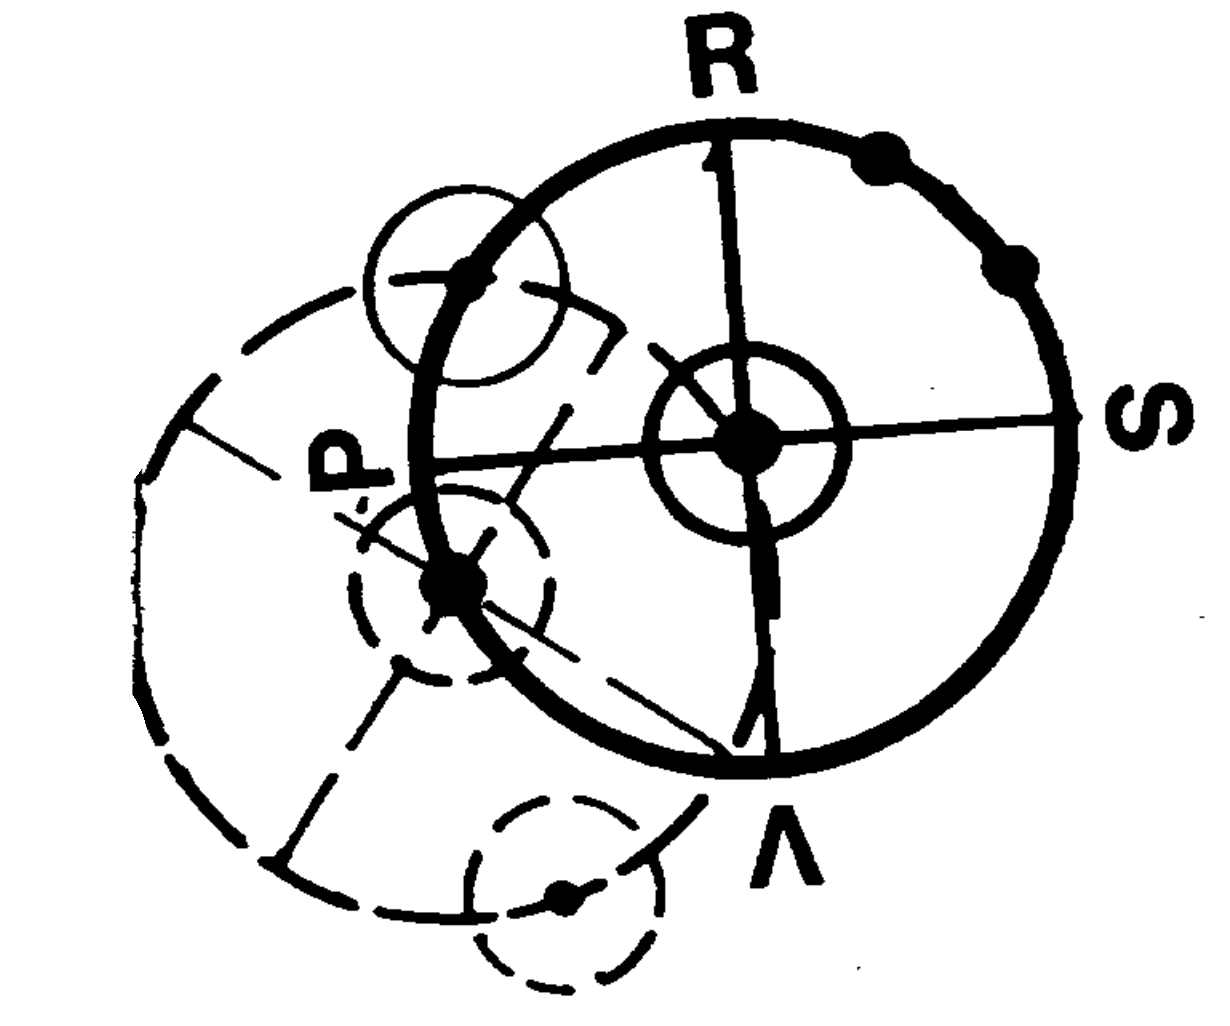
\includegraphics[width=\textwidth]{chapters/3/fig/rvsp_relative.png}               
  \caption{The RVSP cycle changes its position dynamically, relative to the previous state.\cite{halrprin1969rsvp}}
  \label{fig:rvsprelative}
\end{marginfigure}

\textbf{Arata Isozaki}//
Architect Arata Isozaki held an exhibition in 1997 using the internet and email for planning, which is one of the earliest examples of collectively designing an urban scale project by both citizens and professional collaboration with each other. A fictitious island was the site for this design iteration with three methods for this participatory approach; each art piece named `the internet', `visitors' and `signatures.'

`The internet' was the open platform that would let opinions from the public modify the virtual plan. The total number of people connected to the web in Japan was only around 10\% of the \hlcyan{whole country's population}. The exhibition was open for gathering opinions via email and provided 3D models to modify or overwrite the existing design.
\footnote{Information Technology White Paper
\url{http://www.soumu.go.jp/johotsusintokei/whitepaper/ja/h27/html/nc372110.html}}

`Signatures' had 50 architects assigned to a site and separately planned one of their previous architectural pieces without the considerations that are usually sorted out, such as orientation and size. The initial layout plan triggered problems that would need negotiation between adjacent architects to `fit' their design properly. 

`Visitors' focused on the chronological aspect of collaborative design. It had a chief architect that supervised one district for a total of two weeks, passing it to the next architect after their turn. This work flow has similarities in today’s software development, where people collaboratively develop software by forking code made by peers. The architects were encouraged to collect data from the internet. This exhibition was not only novel because of using the internet and email, but was an experiment on how we collaborate and interact using these new techniques.

\hlcyan{Each dealing with mass communication(=`the internet'), negotiation with peer neighbors(=`signatures'), and chronological collaboration(=`visitors'), we see that this exhibition takes collaboration as the central factor, experimenting what will happen when modern technology has been introduced to it.}


\subsection{Browser based applications}

\hlcyan{Browsers are a type of software that arguably have had the most money and effort involved in their development.} Yet ‘browsers’ are particular in ways that are cross platform, including different devices from smart phones to desktop work stations. The following are the web applications I have developed for participatory design.

\textbf{Nigechizu -Shortcut Evacuation Planning \hlcyan{for Tsunamis}-}

\begin{figure}[htb]
  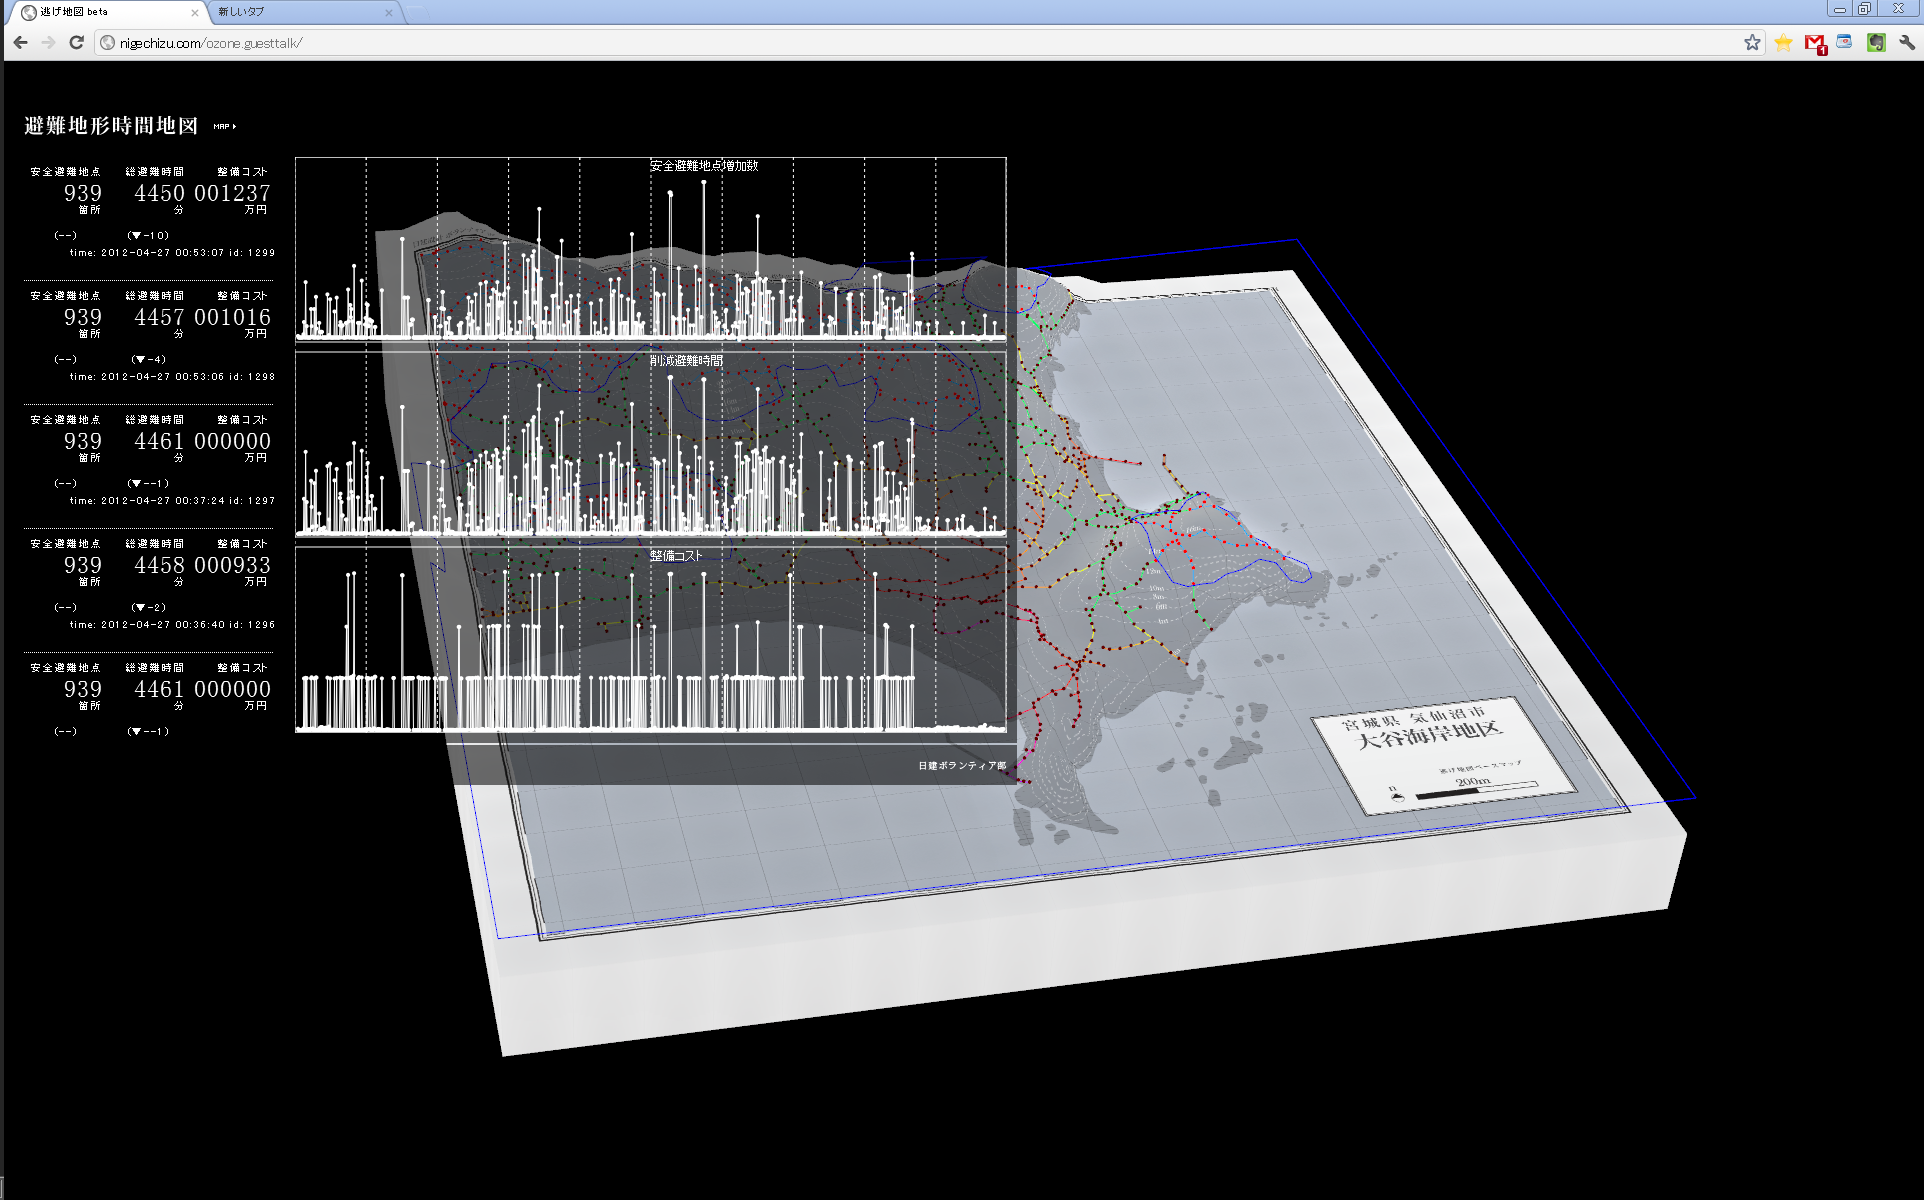
\includegraphics[width=\textwidth]{chapters/3/fig/nigechizu002.png}               
  \caption[nigechizu]{\textfb{Web based short cut planning tool} created for workshops
to learn the risks of tsunamis and how to evacuate.}
  \label{fig:nigechizu}
\end{figure}

As a reaction of the tsunami damage from the 2011 Tohoku earthquake and tsunami, I have created this tool to engage citizens affected by this disaster.

This web browser based tool starts by visualizing the risk of a tsunami coloring the paths depending on the duration for evacuation.
\footnote{This was calculated by a normal walking speed of an elderly citizen, taking the shortest path to the closest high enough altitude.}
After the first strike of the tsunami, people constantly wanted to know which direction to escape because it was sometimes not obvious given the \hlcyan{complex} terrain of the Tohoku region. The second feature was to let the community choose how to create shortcuts. Since shortcut paths reduce the time for evacuation, selecting two points and connecting them increases the area’s safety level as a whole. The significance of this app is enabling people to choose two points to connect, unlike voting for a particular configuration. The trials were recorded in the server to be superimposed to get the most popular positions that needed to be connected.

\begin{marginfigure}[{0cm}]
  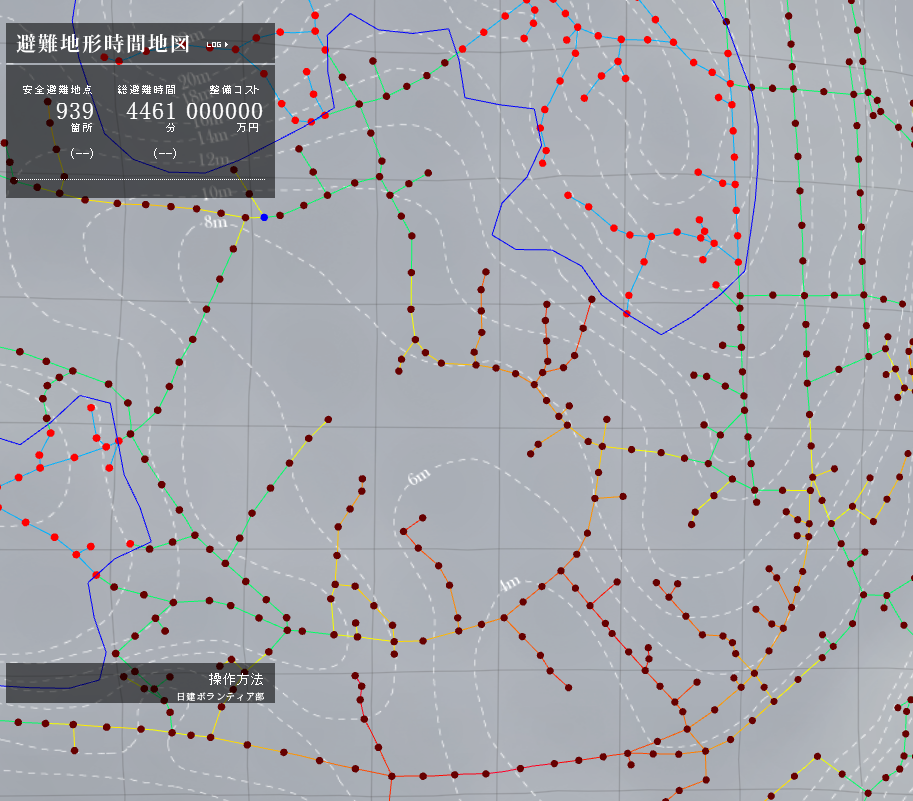
\includegraphics[width=\textwidth]{chapters/3/fig/nigechizu001.png}               
  \caption[zoom in nigechizu interface]{Users will connect two points to create a shortcut to decrease the overall evacuation time.}
  \label{fig:nigechizu}
\end{marginfigure}

\begin{marginfigure}[{0cm}]
  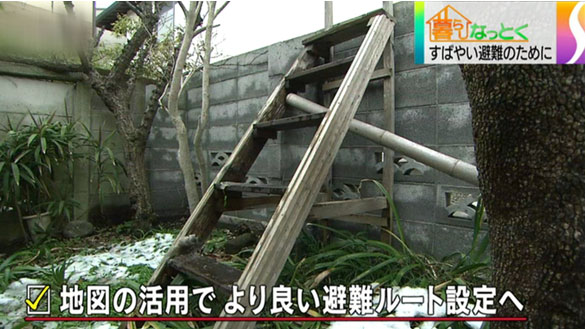
\includegraphics[width=\textwidth]{chapters/3/fig/nhk_kamakura.jpg}               
  \caption[collective collaboration]{After one of the workshops neighbors
  negotiated with each other and installed a wooden staircase to be used as
a general asset for emergency evacuation. \url{https://www3.nhk.or.jp}}
  \label{fig:nigechizu}
\end{marginfigure}


\textbf{LMN Architects -distributed version controlling in 3d
models-}

This example is also a 3d modeling application in a web browser, and every model is connected forming a network. The connection of two models is the inheritance, where the participants choose a preexisting model as a reference and start modeling on top.  The user submits a 3d model, which is a large amount of data compared to voting or connecting dots, and often thought of as unstructured data. The application saves the 3d model into a data structure that could apply a diff algorithm to make the 3d model comparable and calculate the similarities between two models visualizing the strength of the connection.

\begin{figure}[htb]
  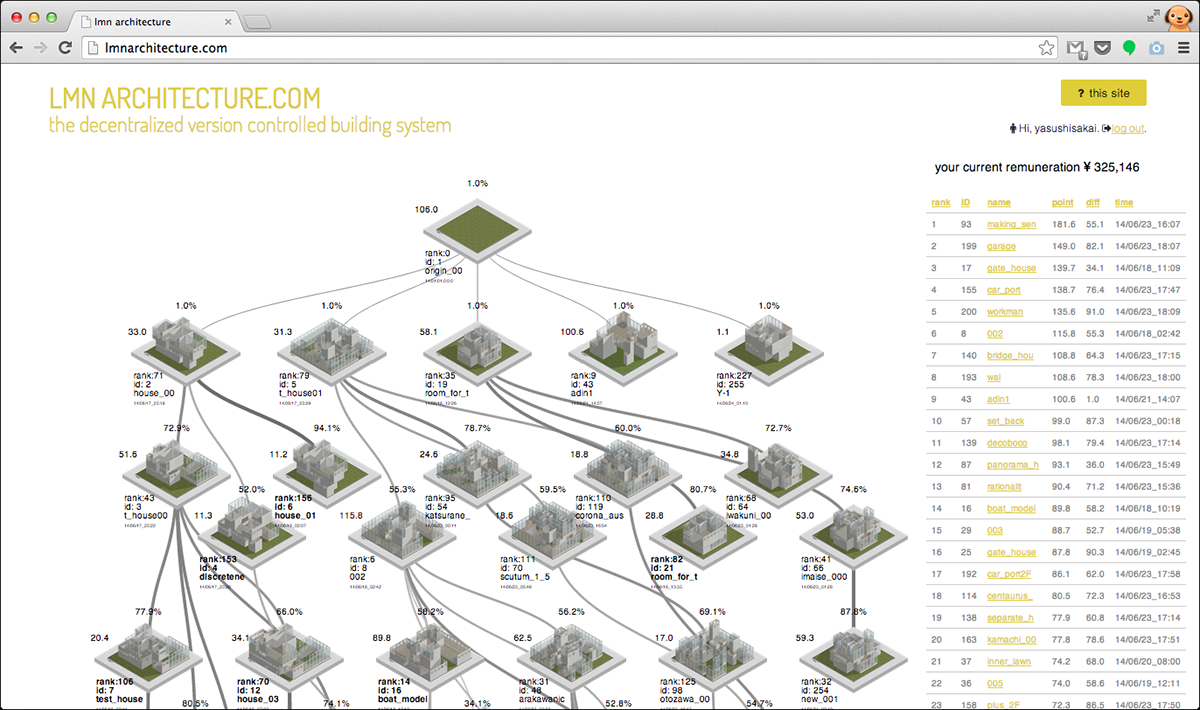
\includegraphics[width=\textwidth]{chapters/3/fig/lmn_004.png}               
  \caption[LMN:web based distributed modelling]{Web based distributed modeling.}
  \label{fig:lnm}
\end{figure}

\begin{marginfigure}[{0cm}]
  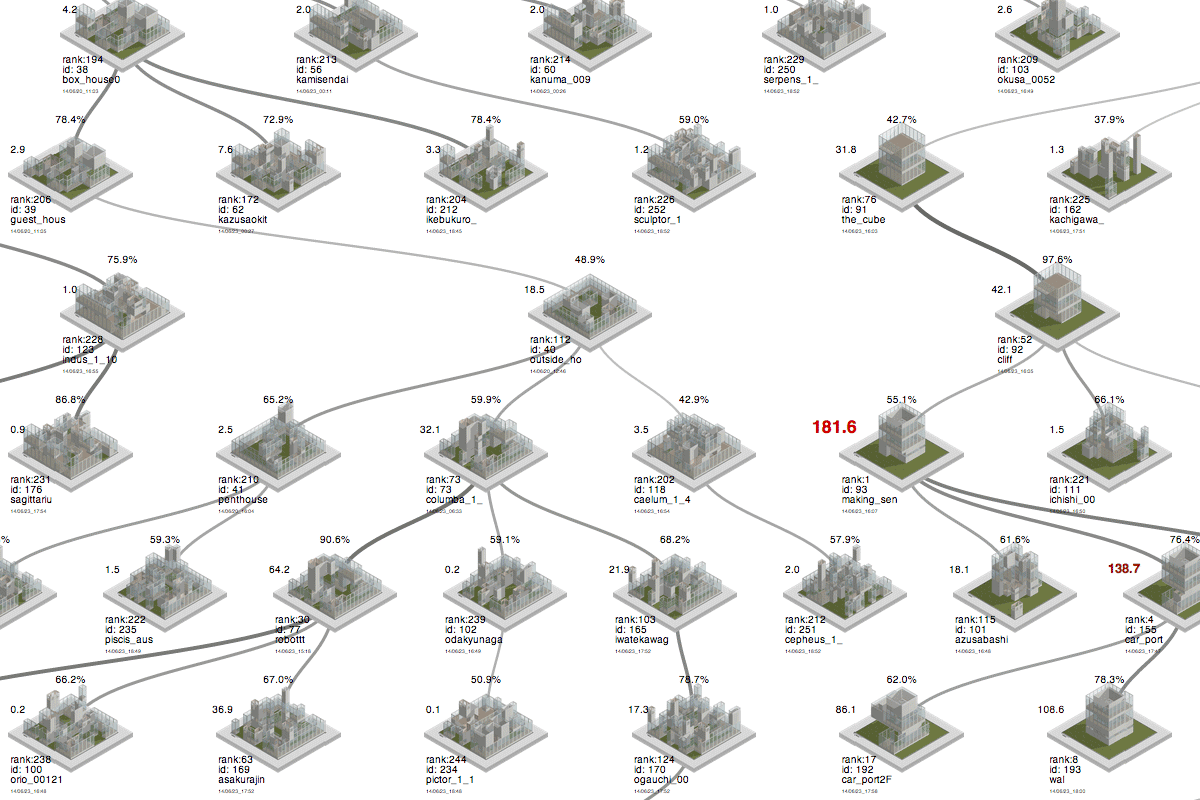
\includegraphics[width=\textwidth]{chapters/3/fig/lmn_000.png}               
  \caption[LMN:net work of models]{Each model starts with a preexisting model and revises it.
Thus, every model is connected, having the similarities calculated by the diff algorithm.}
  \label{fig:lnm_zoom}
\end{marginfigure}

\begin{marginfigure}[{0cm}]
  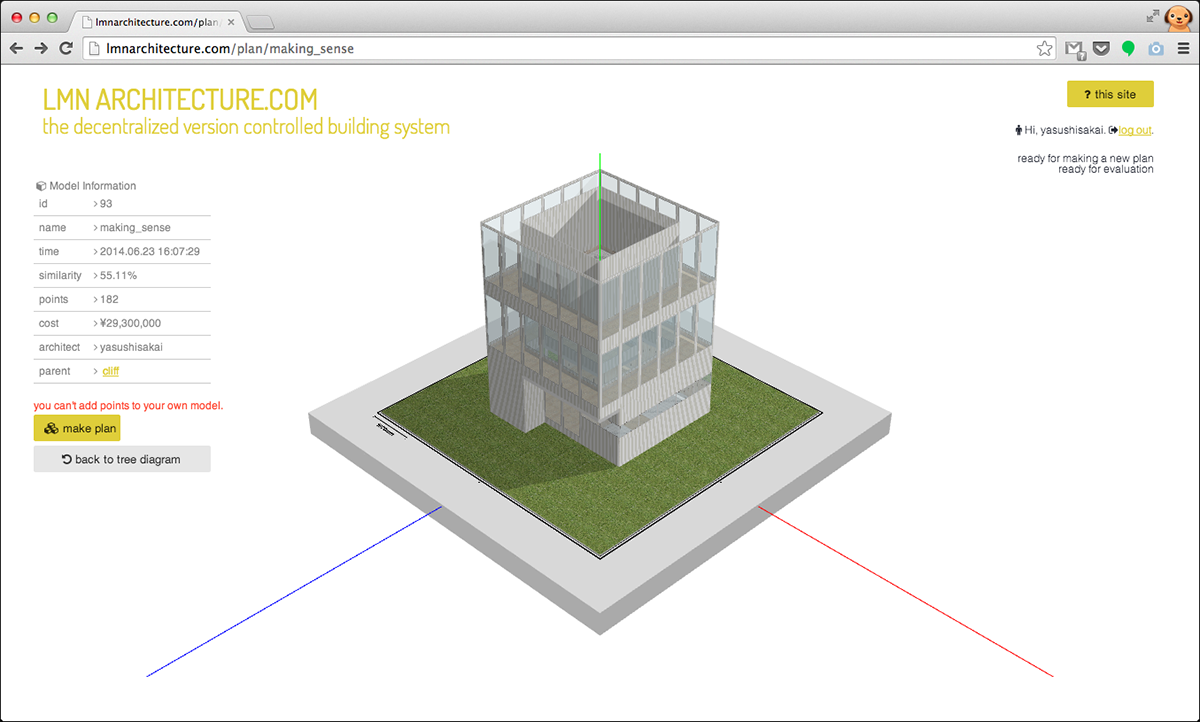
\includegraphics[width=\textwidth]{chapters/3/fig/lmn_006.png}               
  \caption[LMN: modeling inside the browser]{Every model is created using the web browser.}
  \label{fig:lnm_create}
\end{marginfigure}

\textbf{PlacePulse}\\
Place Pulse\footnote{\url{http://pulse.media.mit.edu/}}\cite{salesses2013collaborative} developed by the Collective Learning Group in MIT Media Lab, is a collective effort to map our perception about the city by selecting one image out of two. 10 The amount of information sent per interaction is the smallest in this section, yet has collected more than 1.4 million clicks\footnote{as of August 2017}.

\subsection{Mobile Applications}

\textbf{SeeClickFix}\footnote{\url{https://en.seeclickfix.com/}}\\
\hlcyan{SeeClickFix is a mobile application that is similar to calling the number `311' when citizens demands to report non-emergency maintenance issues. Originally developed for the city of New Haven and has now expanded for more than 300 cities Reporters can submit text and pictures, which is unconstrained. Although not clearly specified, the reports focus on maintenance issues, and less about the planning and changing the city.}

\textbf{Waze}\\
Waze is a driving navigation application, which uses the status of other drivers using the same application. Each driver can passively send the location and speed of the car, or actively contribute to marking the road if there is something worth noting to other drives. Each data is structured. This distributed traffic monitoring is an example of collective analysis, creating mutual benefit and a sense of inclusion between complete strangers who do not share any identity except being drivers. The objective of this application is to form this collective intelligence; there is no connection to any planning procedure.

\textbf{Street Bump} \\
Street Bump developed by the new urban mechanics, is a mobile application that gathers accelerometer data while driving. It is a passive data collection method\footnote{where people do not proactively interact with the data} which is similar to waze, but focused on detecting potholes. The application introduces one question of whether or not we should have the human's fuzziness in the data. In one way, the accuracy of detecting a pothole is a matter of engineering, thus a `tame' problem. Yet we do not know if the human subjects actually cares or feels the pothole is important. In severe cases, people may avoid to step on a pothole, which observation of human behavior is crucial for sensor oriented projects. 
\cite{o2013exploiting}

\textbf{Action Path}\\
Action Path,\footnote{\url{http://actionpath.org/}} \cite{graeff2014crowdsourcing} developed at MIT Center for Civic Media, is a mobile application that shows notifications when a user enters a predefined geolocation and asks questions on urban issues tied to that geolocation. The application provides agency to the citizens and creates data to represent the collective opinion. The interaction with the user produces one of the smallest amounts within this section.

\subsection{Augmentation of Offline community engagement by online tools}

\textbf{Tangible Interfaces: CityScope, Finding Places}\\
City Scope is a platform for people to gather and \hlcyan{build consensus using a device that incorporates data projections}, a tangible interface, and real-time simulation. Multiple projects have advanced using this platform collaboration with different cities and universities. Each project has a different focus, hence the content\footnote{What to visualize/project, type of simulation, who to engage, objective.} has varied.

Finding Places uses City Scope to prove a space for discussing the issue of placing immigrants who’ve come to Hamburg, Germany\footnote{Germany received more than 1.2 million refugees in 2015.}. Using a City Scope table, a total of 34 workshops were conducted to discuss the best place to open room for those seeking asylum. Each session took 2 hours with on average 11 people participating.

This tool covers the analytic phase and synthetic phase and enables people to have real-time feedback running simulations showing potential implications of the population increase. It is a structured tool since users manipulate color coded Lego bricks to run each simulation. On the other hand, the discussion held over the table is rich and vocal.

\begin{figure}[htb]
  
\includegraphics[width=\textwidth]{chapters/3/fig/cityscope.png}               
  \caption[diagram: cityscope]{Changing Places City Scope Platform.}
  \label{fig:diagram_cityscope}
\end{figure}

\textbf{Community PlanIt} \\
Community PlanIt\footnote{\url{https://elab.emerson.edu/projects/civic-media/community-planit}} developed by the Engagement Lab is gaming platform to support civic participation in planning projects.
The platform asks questions or missions to the participant inducing conversation with each other or manifest each others vision for the city. The platform can be used parallel with public meetings that will foster the deliberation process of the event.

\hlcyan{

\textbf{Cambridge participatory budgeting} \\
Participatory budgeting originated in 1989 Brazil, is a bottom up method that people propose and decide how to spend a portion of public tax revenue. Cambridge has been conducting this project, with browser apps augmenting the process. The application has two views: the map and the list. Them map is plot of different proposals that was submitted by other citizens. Users can explore different proposals within their neighborhood. The list has the same information but is sorted by the attention the project has collected.

\textbf{coUrbanize}\footnote{\url{https://courbanize.com/}} \\
This is online platform for urban planners and real estate developers to post their projects and host discussions to gain feedback. The tool is more a platform to list different development projects.

\textbf{tools from delib} \\
Delib \footnote{\url{http://www.delib.net/}} developed a series of online platforms for different occasions necessary for planning and community engagement: `Dialogue' is for project manifestation for gaining feed back of plan proposals, `Citizens Place' is for consolidating questionnaires and online consultations, and `Budget Simulator' is for engaging citizens to gain insights on projects with budgets taken into consideration.
}
